\section{Analyse}

\subsection{Partie 1}
Cette partie était principalement une marche à suivre. Il n'y avait pas réellement d'analyse à effectuer sur cette partie du laboratoire. Le but était de suivre la marche à suivre et de comprendre les actions que nous réalisions.
\subsection{Partie 2}
Cette partie nous demandais d'ajouter la gestion des leds et des afficheurs 7 segments en fonction des switchs et sans gérer pour le moment les interruptions (Key2 et Key3). Ce qui est intéressant dans cette partie, c'est l'ajout des Keys et des afficheurs 7 segments en tant que PIO, en se servant de l'expérience reçu lors de la réalisation de la première partie.
\subsection{Partie 3}
Cette partie demandais un peu plus d'analyses que les deux parties précédentes. Il n'y avait pas de PIO à ajouter, par contre la gestion des interruptions devait être mise en place pour chacun des différents éléments du système. Ainsi, il falait prendre en compte le CPU, le GIC et les PIO.\\ Pour ce qui concerne le CPU, la configuration des vecteurs d'interruptions était fournie, mais la routine d'interruption devait être implémentée.\\ Concernant le GIC, je me suis inspiré des exemples de codes fournis dans le document "Gic\_Altera\_Manuel\_short.pdf", et j'ai dû comprendre comment configurer le GIC. Voici les registres du GIC qui ont dû être configurés ou qui ont été utilisés lors de la routine d'interruption : \\

\begin{itemize}
	\item ICCICR : Permet d'activer la transmission depuis le CPU interface jusqu'au CPU lui correspondant. C'est un enable.
	\item ICCPMR : Permet de set la priorité minimale pour qu'une interruption soit transmise au CPU.
	\item ICCIAR : Lors d'une interruption, contient l'ID de l'interruption en question.
	\item ICCEOIR : Permet au processeur de clear l'interrupt en écrivant l'ID correspondant à l'intérieur
	\item ICDDCR : Permet d'activer le distributor. C'est un enable.
    \item ICDISER : Permet d'activer une interruption (unmask)
	\item ICDIPTR : Permet de définir vers quel CPU doit être envoyé l'interruption.\\
\end{itemize}

A cela s'ajoutait deux registre , KEYS\_INTERRUPT\_ENABLE et\\ KEY\_INTERRUPT\_REGISTER, qui permettait d'activer les interruptions des keys dans la FPGA et de récupérer ainsi que nettoyer lesdites interruptions.\\

Nous parlerons des valeurs qui ont été attribué à chaque registres dans la partie implémentation. Les adresses des registres sont basés sur les calculs fournis dans la documentation en fonction du numéro d'interruption 72, qui correspond au numéro d'interruption 0 de la FPGA (Nous verrons dans la partie implémentation d'ou vient ce numéro).

\subsection{Adress Map finale}

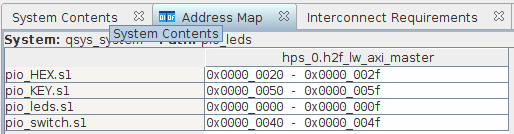
\includegraphics[scale=0.6]{./images/address_map.png}
\captionof{figure}{Laboratoire 2 : Address map}
\par
Le choix des offsets ci-dessus vient à la base d'un problème de compréhension. J'avais choisi ces offsets en fonction des adresses correspondantes dans le memory layout fournit dans le document "DE1-SoC\_Computer\_ARM.pdf". Si cela n'apporte pas de problème en tant que tel, il faut tout de même noter que j'aurais pu en choisir d'autres, en faisant en sorte qu'ils soient contiguë par exemple.

